\chapter{State of the art modelling of comfort}
\label{cha:Literature_study}
As discussed in the introduction, the goal of this thesis is to implement a method to capture personal experience of comfort during driving. This will be done by using inverse optimal control where the weighting factors in the objective function are learned from demonstration. A literature study was needed to understand how comfort is defined and how the inverse optimal control method can be implemented.\\

This chapter is structured as follows. First, the definition of comfortable driving is looked into in section \ref{s:comfort_parameters}. Section \ref{s:inverse re le} concerns a discussion of the inverse optimal control concept used.

\section{What is comfort during driving?}
\label{s:comfort_parameters}
In the US patent of L. Daniel \cite{Daniel2018}, the idea is to assess the amount of comfort by calculating a value for carsickness. This value is calculated by a weighted sum of sway motion, surge motion and heave motion of the vehicle. These motions are being directly calculated from the lateral acceleration, fore-aft acceleration and the vertical acceleration of the vehicle. \\

\begin{figure}[h!]
	\centering
	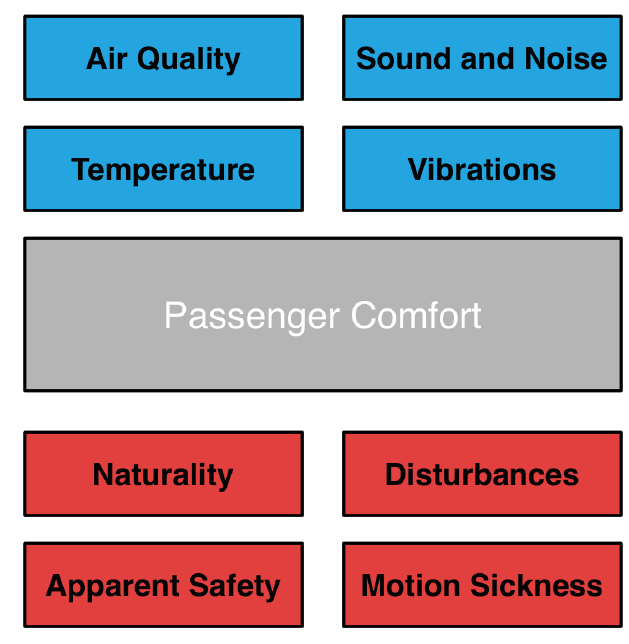
\includegraphics[width=0.48\textwidth]{comfort.PNG}
	\caption{Overview of comfort parameters in autonomous vehicle with old parameters (blue) and new ones (red).(Source: \cite{Elbanhawi2015})}
	\label{fig:Comfort}
\end{figure} 

%\begin{wrapfigure}[22]{L}{0.5\textwidth}
%	\begin{center}
%		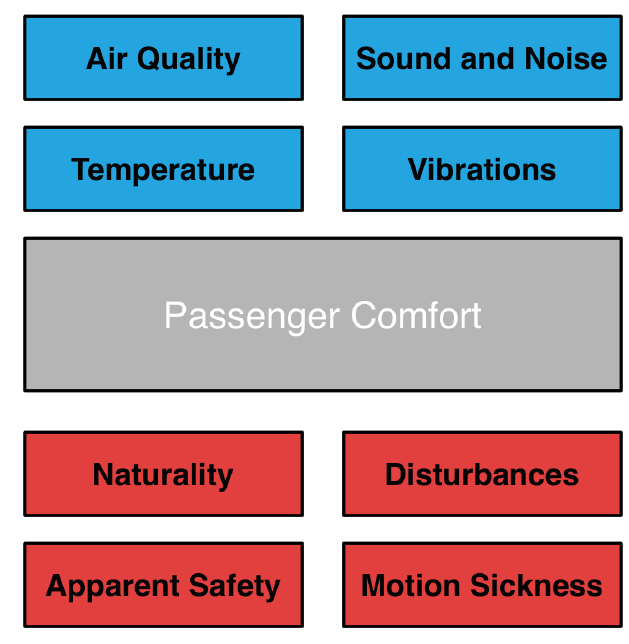
\includegraphics[width=0.48\textwidth]{comfort.PNG}
%	\end{center}
%	\caption{Overview of comfort parameters in autonomous vehicle with old parameters (blue) and new ones (red).(Source: \cite{Elbanhawi2015})}
%	\label{fig:Comfort}
%\end{wrapfigure}
In the paper 'Investigating ride comfort measures in autonomous cars' \cite{Elbanhawi2015}, it is explained that due to the introduction of autonomous vehicles there will be an other perception of comfort. Figure \ref{fig:Comfort} indicates in blue the claimed traditional comfort factors and in red the new ones that additionally have to be taken into account when driving in autonomous vehicles. Concretely this can be translated into the preference of smooth trajectories and low lateral motions when the roads are assumed to be sufficiently smooth. A hypothesis taken, is that motion sickness will be more prominent in autonomous driving due to the loss of control. It is also argued that the distance to an obstacle is contributing to a comfortable feeling.\\

In 'Analysis of Driving Style Preference in Automated Driving' \cite{Bellem}, three studies were completed to capture the definition of comfortable driving in autonomous vehicles.\\
During the first study, human drivers drove manually with their own driving style a set of maneuvers and in this data, there was sought after relevant metrics that could be used to define comfortable driving. The results of this research was that accelerations play a key role in comfort but are not the only factor \cite{Bellem}.

\begin{quote}
	The different comfort metrics found were:
	\begin{itemize}
		\item lateral and longitudinal acceleration;
		\item lateral and longitudinal jerk;
		\item quickness of the maneuver;
		\item headway distance;
	\end{itemize}
\end{quote}

Quickness of the maneuver indicates that it is received as comfortable when the vehicle gives a good response and reaches the desired lateral displacement faster.
Additionally comfortable driving as assessed in \cite{Bellem}, can be summarized as  sufficiently smooth trajectories and keeping enough headway distance in order to have a feeling of control and safety. These results suggest that when an algorithm is evaluating comfort, a notion of the surrounding traffic should be present. It was found when the traffic density on the road is higher, the driver is more tolerant towards less smooth driving behaviour e.g. to be able to insert in a busy lane. In this case higher comfort can be attained if the driver has the feeling of a fast response of the vehicle, translating in early peaks of acceleration. Vertical vibrations are outside the scope when roads are assumed sufficiently smooth.\\

In a second study the main metrics found from study one are rated making use of a questionnaire, asking about the amount of comfort retrieved. ''Out of this it followed that accelerations are again playing a key factor'', according to paper \cite{Bellem}. For lane changes it could be concluded that maneuvers with a small lateral acceleration and early perceivable onset were more comfortable.\\

That also jerk plays an important role in the attained amount of comfort, is confirmed by paper \cite{Gianna1996} where it is stated that: ''Jerk has been shown to elicit a stronger influence on comfort than acceleration''.


% In mijn maneuver wordt de kleine waardes van longitudinale snelheid en versnellingen gecompenseerd door de normalisatie waarden. Dus ookal zijn ze klein, krijgen toch een grote impact mee in het berekenen van een optimale oplossing. Daarin tegen kan er wel makkelijker voldaan worden aan het perfect voldoen van de longitudinale parameters in de lane change zonder het algemene resultaat veel te veranderen. De keuzen van de wegingsfactoren worden hierdoor minder significant en sensitiviteit wordt lager. --> als verschillende maneuvers worden gecombineerd zal dit de uniekheid van de gevonden wegingsfactoren opdrijven.

%Zie quotes van de slides!

\section{Inverse optimal control}
\label{s:inverse re le}
Because every human has its own driving style, it is a cumbersome task to tune the weighting factors of an objective function for each individual in order to model a personal perception of comfort. In paper \cite{Powers} it is showed that manual tuned weighting factors will besides lead  to suboptimal solutions in comparison with learned ones from data. 
Inverse optimal control is the activity of learning an agent's objective function from expert demonstrations \cite{Arenz2017}.\\

The goal of the learning algorithm explained in this thesis is to derive the weighting factors $\theta_j$ of different linearly combined comfort criteria $f_j$, embedded in the cost function $J$. As the observed data is explained better during learning, it is assumed that $J$ is getting closer to the inner comfort objective of the individual driver. However, it should be noted that the driver takes unknowingly a lot of comfort criteria into account and they are not all linearly related as is suggested by Eq. (\ref{eq:1}). Therefore the comfort cost function in Eq. (\ref{eq:1}), will always be an approximation of reality. Although as discussed in paper \cite{Kuderer2015a}, it is possible to capture the magnitude of the main contributors of comfort experienced by the users\\

\begin{equation}\label{eq:1}
	J = \sum_{j=1}^{Z}\theta_j\cdot f_j	.
\end{equation}

%"Inverse optimal control, also known as inverse reinforcement learning, is the problem of recovering an unknown reward function in a Markov decision process from expert demonstrations of the optimal policy." \cite{Levine2012} In contrary what this classic definition, the approach followed by \cite{Kuderer2015a} is not modelling teh

In order to create a generative model that creates vehicle paths $\bm{r}_i$ with equivalent kinematic characteristics as the path that was observed $\bm{r}_{obs,i}$, a feature-based inverse optimal control is applied, with $i \in [1 ... m]$ and $m$ the amount of observed trajectories \cite{Kuderer2015a,Abbeel2004}. A feature is encoding relevant kinematic properties onto a scalar value and the difference between the demonstrated and calculated feature values, give an indication about the similarity of the kinematic signals i.e. displacement, velocity, acceleration and jerk. \\

\subsection{Feature-based inverse optimal control}
A feature value maps a signal onto a scalar and encapsulates a comfort criteria. The higher the scalar value the more discomfort is experienced by the driver. An example is given by Eq. (\ref{eq:3}) that measures the amount of accelerations in a maneuver

\begin{equation}\label{eq:3}
f_j:\bm{r}\xrightarrow{}f_j(\bm{r})=\int_{0}^{T}a_x(t)^{2}+a_y(t)^{2} dt.
\end{equation}
The different feature values are collected in a feature vector $\bm{F} \in \mathbb{R}^Z$ with on its entries the different feature values $f_j$.
The path that is followed by the vehicle is represented by $\bm{r}$.

%the centre of gravity of the vehicle is following can be represented by Eq. (\ref{eq:4}).
%\begin{equation}\label{eq:4}
%\bm{r}:t \xrightarrow{}\bm{r}(t) =  \bigl( \begin{smallmatrix} x(t)\\ y(t) \end{smallmatrix}\bigr)
%\end{equation}

The human driver is not a deterministic agent and is modelled by a stochastic distribution $p(\bm{r}|\bm{\theta})$. For certain weighting factors $\bm{\theta} \in \mathbb{R}^Z$ a path $\bm{r}$ is produced as being a sample of a stochastic distribution. The distribution chosen, is the distribution of maximum entropy Eq. (\ref{eq:entropy}) as suggested in paper \cite{Ziebart2008}. When using the maximum entropy distribution the amount of prior information embedded in the distribution is minimized. It is also stated that many physical systems will move towards a maximal entropy configuration over time
%''The distribution with the highest entropy represents the given information best since it does not favour any particular outcome besides the observed constraints'', according to \cite{Abbeel2004}.
	
\begin{equation}\label{eq:entropy}
	p(\bm{r}|\bm{\theta}) = exp(-\bm{\theta}^T\cdot \bm{F}(\bm{r})).
\end{equation}
Eq. (\ref{eq:entropy}) can be interpreted as a cost function $\bm{\theta}^T\bm{F}(\bm{r})$ where agents are exponentially more likely to select trajectories with a lower cost which is felt as more comfortable \cite{Kuderer2015a}.
%The averaged observed feature vector is $\til{\bm{F}}_{av} = \frac{1}{m}\sum_{j=1}^{m}\til{\bm{F}_j}$.\\

In order to explain the observed feature vector $\bm{F}_{obs}$, the weighting factors $\bm{\theta}$ need to be found that match the expected feature vector $\bm{F}(\bm{r}_{expected})$ with $\bm{F}_{obs}$. The observed feature vector $\bm{F}_{obs} \in \mathbb{R}^Z$ has on its entries the different feature values $f_{obs,j}$. $\bm{r}_{expected}$ is defined as $ E(p(\bm{r}|\bm{\theta}))$. To go towards a match with the observed feature vector, a gradient descent method can be used with as estimation of the gradient $\pdv{\bm{F}_{diff}}{\bm{\theta}}$ by $\bm{F}_{obs} - \bm{F}(\bm{r}_{expected})$ and with $\bm{F}_{diff}$ the difference between the feature vectors \cite{Ziebart2008, Kretzschmar2014}. Only the sign of the gradient is used and there are two directions for every weighting factor update: increase or decrease. Therefore an intuitive explanation exist for using $\bm{F}_{obs} - \bm{F}(\bm{r}_{expected})$ as estimation for the gradient. The weighting factor is increased when the expected feature is higher than the observed one, which means that the associated comfort feature will be punished more severely in Eq. (\ref{eq:entropy}) and paths with a higher value of that comfort feature become less likely. The weighting factor will be decreased when the expected feature is lower than the observed one \cite{Kuderer2015a}. Eq. (\ref{eq:5}) summarizes the gradient descent method with $\alpha$ the step size taken in the direction of descent

\begin{equation}\label{eq:5}
	\bm{\theta}^{k+1} = \bm{\theta}^{k} - \alpha \pdv{\bm{F}_{diff}}{\bm{\theta}}^k .
\end{equation}

When $\bm{\theta}_{optimal}$ is found the gradient is minimized and the feature vectors will match as closely as possible. In order to achieve this, the problem remains how to retrieve $\bm{F}(\bm{r}_{expected})$. In order to calculate $\bm{F}(\bm{r}_{expected})$ a Hamiltonian Markov chain
Monte Carlo stochastic distribution sampling method was used in paper \cite{Kretzschmar2014}. In paper \cite{Kuderer2015a} a simplified and less calculation demanding approach is proposed, where it is assumed that the expected path is also the one that is been assessed as the most comfortable by the human driver. The path that is perceived as the most comfortable can be estimated by minimizing Eq. (\ref{eq:1}) for certain weighting factors. Equation \ref{eq:6} summarizes the method proposed by paper \cite{Kuderer2015a}
\newcommand{\argmax}{argmax}
\newcommand{\argmin}{argmin}
\begin{subequations}
	\label{eq:6}
\begin{equation}\label{eq:6a}
	\bm{r}_{expected} = \underset{\bm{r}}{\argmax} \hspace{1mm} p(\bm{r}|\bm{\theta}) = \underset{\bm{r}}{\argmin} \hspace{1mm}  \bm{\theta}^T\cdot \bm{F}(\bm{r}),
\end{equation}
\begin{equation}\label{eq:new}
	\pdv{\bm{F}_{diff}}{\bm{\theta}} = \bm{F}_{obs} - \bm{F}(\bm{r}_{expected}).
\end{equation}
\end{subequations}

%\DeclareMathOperator*{\argmin}{argmin}

\subsection{RPROP algorithm}\label{s:RPROP}
From reference \cite{Panos_opti} it is known that not every step size of the gradient is leading to convergence towards a minimum. When the step size is too small, it will take a long time to converge. However when it is chosen too big, cycling behaviour between limit points occurs. In order to avoid this unwanted behaviour, a  method is needed to change the step size taken during the course of the algorithm. For this the resilient backpropagation algorithm (RPROP) \cite{RPROP} is used as it was first proposed by Martin Riedmiller and Heinrich Braun in 1993.\\

The main advantage when using RPROP is that the size of the gradient is not blurring the update value of the weighting factors. The update value $\Delta u$ is solely dependent on the sign of the current gradient, the sign of the gradient in the previous iteration and the update value in the previous iteration. The three possible cases for the update value during iteration $t$ are given by: 

\begin{equation}\label{eq:7}
	\Delta u^t_j =
	\begin{Bmatrix}
		 \eta^+ \cdot \Delta u^{t-1}_j, & if \hspace{1 mm} \pdv{f_j}{\theta_j}^t \cdot \pdv{f_j}{\theta_j}^{t-1} > 0 \\
		 \eta^- \cdot \Delta u^{t-1}_j, & if \hspace{1 mm} \pdv{f_j}{\theta_j}^t \cdot \pdv{f_j}{\theta_j}^{t-1} < 0 \\
		  \Delta u^{t-1}_j, & if \hspace{1 mm} \pdv{f_j}{\theta_j}^t \cdot \pdv{f_j}{\theta_j}^{t-1} = 0 \\
	\end{Bmatrix}.
\end{equation}
\begin{equation}\label{eq:9}
0 <\eta^-<1<\eta^+
\end{equation}

When the update value of the weighting factor is determined, it is applied in the direction of steepest descent which equals the opposite direction of the current gradient

\begin{equation}\label{eq:8}
\Delta \theta^t_j =
\begin{Bmatrix}
	-\Delta u^t_j, & if \hspace{1 mm} \pdv{f_j}{\theta_j}^t > 0 \\
	+ \Delta u^t_j, & if \hspace{1 mm} \pdv{f_j}{\theta_j}^t < 0 \\
	0, & else 
\end{Bmatrix}.
\end{equation}
Exception on Eq. (\ref{eq:8}):

\begin{equation}\label{eq:10}
	\Delta \theta^t_j = -\Delta \theta^{t-1}_j, \hspace{1mm} if \hspace{1mm} \pdv{f_j}{\theta_j}^t \cdot \pdv{f_j}{\theta_j}^{t-1} < 0.
\end{equation}



With $\theta_j^{t+1} = \theta_j^{t} + \Delta \theta^t_j$, $j \in \mathbb{N}_{[1\cdots Z]}$ and $t \in \mathbb{N}_{[1 \cdots \mathbb{\tau}]}$ the amount of iterations. Every time the partial derivative $\pdv{f_j}{\theta_j}^t$ of the corresponding weighting factor $\theta_j^t$ changes its sign, it is assumed that the last update was too big and the local minimum was passed. In Eq. (\ref{eq:7}) the step size is then reduced and in order to go back to the previous situation the update of the weighting factor is done as indicated by Eq. (\ref{eq:10}). To not again decrease the update value when going back to the previous situation where the gradient will again change it's sign,  $\pdv{f_j}{\theta_j}^{t}$ is set to zero.\\
If the derivative retains its sign with respect to the previous iteration, the update value is slightly increased in order to accelerate convergence in shallow regions \cite{RPROP}. Parameters set by the user are: $\Delta u^0_j,\Delta u^{max}_j,\Delta u^{min}_j, \eta^+$ and $\eta^-$. In this thesis following values were chosen: $\Delta u^0_j = 0.1$, $\Delta u^{max}_j=1.0$, $\Delta u^{min}_j=10^{-7}$, $\eta^+ = 1.2$ and $\eta^- = 0.5$.

%e the assumption of calculating most likely path --> features expected = f(r_exp) instead of sampling as is done in this paper.
%(Hamiltonian Markov chain Monte Carlo methods = very computation expensive)
%



%When the averaged observed feature vector $F$
%
%In order to be able to explain the observed trajectory
%
% Firstly he is generating observed paths that are a sample of a distribution and secondly he is minimizing its own comfort cost function.
%
% 
%The exponential distribution is giving a higher chance to produce paths that have a low feature value associated  with a high weight factor. This means that the more influence a feature value has on the total amount of comfort (higher weight), how less likely it becomes that the driver will produce a certain path that will trigger a high value of the concerned feature value. 
%
%If you maximize the probability you get the most likely expected path for the chosen weighting factors.  This can be translated in the assumption that the driver is most likely to produce a path that will be experienced as comfortable as possible by himself. The assumption that the driver is optimizing its own comfort cost function is an assumption on top of assuming that the observed path is a sample of an exponential distribution with certain weight factors. 
%
%The goal of the learning process is to learn the model parameters (weight factors) of the driver from their observed driving style. It is assumed that the driver can be explained by a probability distribution and that it produces paths that minimize a comfort cost function. When the comfort model of the driver is learned, it can be further used in general situations. This is done by implementing the user specific notion of comfort in the motion planning algorithm of a model predictive control planning application.
%
%The learned model should produce trajectories that are similar in order of comfort as experienced by the driver. This is a logical consequence because the model is derived from the observed data. The difference between the features of the observed and generated paths quantify the similarity and at convergence of the learning algorithm, the feature values are as close as possible. As close as possible should be taken with a grain of salt though. This can be explained by making a comparison between the curvature and the jerk where curvature is in order of 10^-5 and jerk is in order of 10^2. This means that a difference of 1 has a far more bigger impact on curvature than on jerk and normalization is necessary. Normalization is done by dividing the calculated features by their corresponding observed feature value in order to make it dimensionless.  This means that the optimization should be done without fixing time! The difference in feature values is the driving factor and this will indirect specify also the time of the lane change.
%
%Learning a model implies finding the best suitable values of the tunable parameters which are in this case the weight factors. To summarize, the goal of the learning algorithm is to find the weight factors which give the smallest difference between the feature values of the observed path and the feature values of the calculated path, which is the path that minimizes the linear comfort cost function. The calculated path is generated by the minimization of the comfort cost because minimizing the comfort cost function is equal to maximizing the exponential distribution and the resulting path is equal to the most likely generated path for certain weight factors. The most likely generated path is compared with the observed one. With this it is indirectly assumed that the observed paths are generated by a human driver that is minimizing its own unknow comfort cost function. It will be clear from the validation in chapter \ref{} if this assumption holds. From [hoofdrapport] it is assumed that this approximation is suitable in the context of learning individual driving styles on highways.  Two assumptions apply on the human driver. Firstly he is generating observed paths that are a sample of a distribution and secondly he is minimizing its own comfort cost function. It should be noted that in practice instead of using personal data also data form an expert driver can be made available to the user. This to avoid bad autonomous behavior as a result of an inexperienced human driver.
%
%
%Note that the features of the path that are obtained by minimizing the comfort cost function should be possible to converge to the features of the observed path. The driver that is producing the observed path is assumed to maximize its personal comfort when generating the observation data which means that the most personal comfort is attained when the difference between the feature values of the observed and calculated paths are small. (this should be normalized) 
%


\section{Conclusion}
In order to identify comfort criteria during driving, a literature study was conducted which was mainly questionnaire based. The results were that to be able to evaluate comfort, higher order kinematic variables like accelerations and jerks must be considered. These variables are important to acquire a smooth vehicle path and to give a continuous and natural feeling when driving. The quickness of the maneuver and the feeling of save driving should also be taken into account. Therefore comfort is naturally influenced by the environment of the vehicle. It was found that when more traffic is present, a higher tolerance for less smooth trajectories is granted. Finally, it was explained that if the goal of the maneuver is more rapidly completed, this influences the amount of comfort in a positive way.\\

In the second part of the literature study the concept of inverse optimal control was clarified and it was explained that it is the process of identifying the unknown objective of the human driver. Next, feature based learning has been looked into and a practical method was found in order to retrieve $\bm{\theta}_{opti}$ making use of gradient descent. After this the RPROP algorithm was introduced that will be used to update the weighting factors while making use of the gradient descent method in order to match expected feature values with the observed ones.

\newpage


%\section{bekijk hiervoor de andere approaches - to be read further}
%
%\subsection{Machine learning approach}
%\subsection{paper brecht approach}

%Dan komt de vraag wat is comfort precies? Literatuur studie...
%Waarnaar kan men kijken als men het over comfort heeft. 
%Lane change bekeken om comfort te valideren --> zeg dat er geen iso standaarden aanwezig zijn.
%Hoe wordt een bestuurder gemoddelleerd --> dit wordt gedaan door een kansverdeling.
%Waarom is entropie nuttig om deze bestuurder te kunnen bekijken? Doe hier meer ondezoek over en verantwoord het gebruik hiervan. Conclusie komt af met comfort parameters die verder worden gebruikt als features.
%Bij de uitleg van de features en waarom er versnelling en acceleratie wordt gebruikt, basseer ook op paper 7 van hoofdpaper--> geen acces
%
%Wat wordt er in de literatuur al gebruikt om comfort te modelleren en geef een overzicht.
%
%Leg uit hoe komt aan entropy distribution komt --> kan beroep doen op ref 2 en 20 van het hoofdrapport (both are assuming an exponential distribution) (IMPORTANT) --> literatuur study niet te uitgebreid maken...
%
%Check uitgebreide samenvatting van hoofdpaper op oneNote.
%
%Dit is de reden voor het gebruik van de maximum entropie distributie: 
%	To learn observed behavior, we aim to model the distribution
%	that underlies the empirical sample trajectories.
%	Following Abbeel and Ng [1], we aim to find a model that
%	induces distributions that match, in expectation, the feature
%	values fD of the empirical trajectories D, yielding
%	Ep(x)[f (x)] = fD =
%	1
%	jDj
%	X
%	xk2D
%	f (xk): (1)
%	In general, however, there is not a unique distribution that
%	matches the features. Ziebart et al. [24] resolve this ambiguity
%	by applying the principle of maximum entropy [10], which
%	states that the distribution with the highest entropy represents
%	the given information best since it does not favor any
%	particular outcome besides the observed constraints. (this is the least baised distribution)
%	Modelling expected featueres by hybrid monte carlo method: https://reader.elsevier.com/reader/sd/pii/037026938791197X?token=71567B7640C402F2FF578E34E3BB7914CA14E4A1A29DE88D9534D96C9305E13DA52D0424FF1475A822FCE784725196D3
%%	ref: C:\Users\t2vosx\OneDrive\Documenten\Leuven\Thesis\References2\Citations on main %paper\Learning to Predict Trajectories of Cooperatively Navigating Agents.pdf>
%
% 	paper: Feature-based prediction of trajectories for socially compliant navigation
%	which
%	states that the distribution with the highest entropy represents
%	the given information best since it does not favor any
%	particular outcome besides the observed constraints.
	
%	• Weet dat exponentiële vorm oplossing is van boven staand optimizatie probleem. zie foto
%	--> volgt uit FONC --> oplossing moet (non convex) voldoen aan KKT conditions. Er zijn enkel maar equality constraints aanwezig --> primal feasibility en lagrange stationarity moeten voldaan worden --> LS wordt gecontroleerd drm van de Euler - lagrange vergelijking te gebruiken. 


%%% Local Variables: 
%%% mode: latex
%%% TeX-master: "thesis"
%%% End: 
